\graphicspath{ {./images} }

%!TEX root = ../thesis.tex
\chapter{Methods}
\label{ch:methods}

\section{The Simulink Model}
\begin{figure}
	\centerline{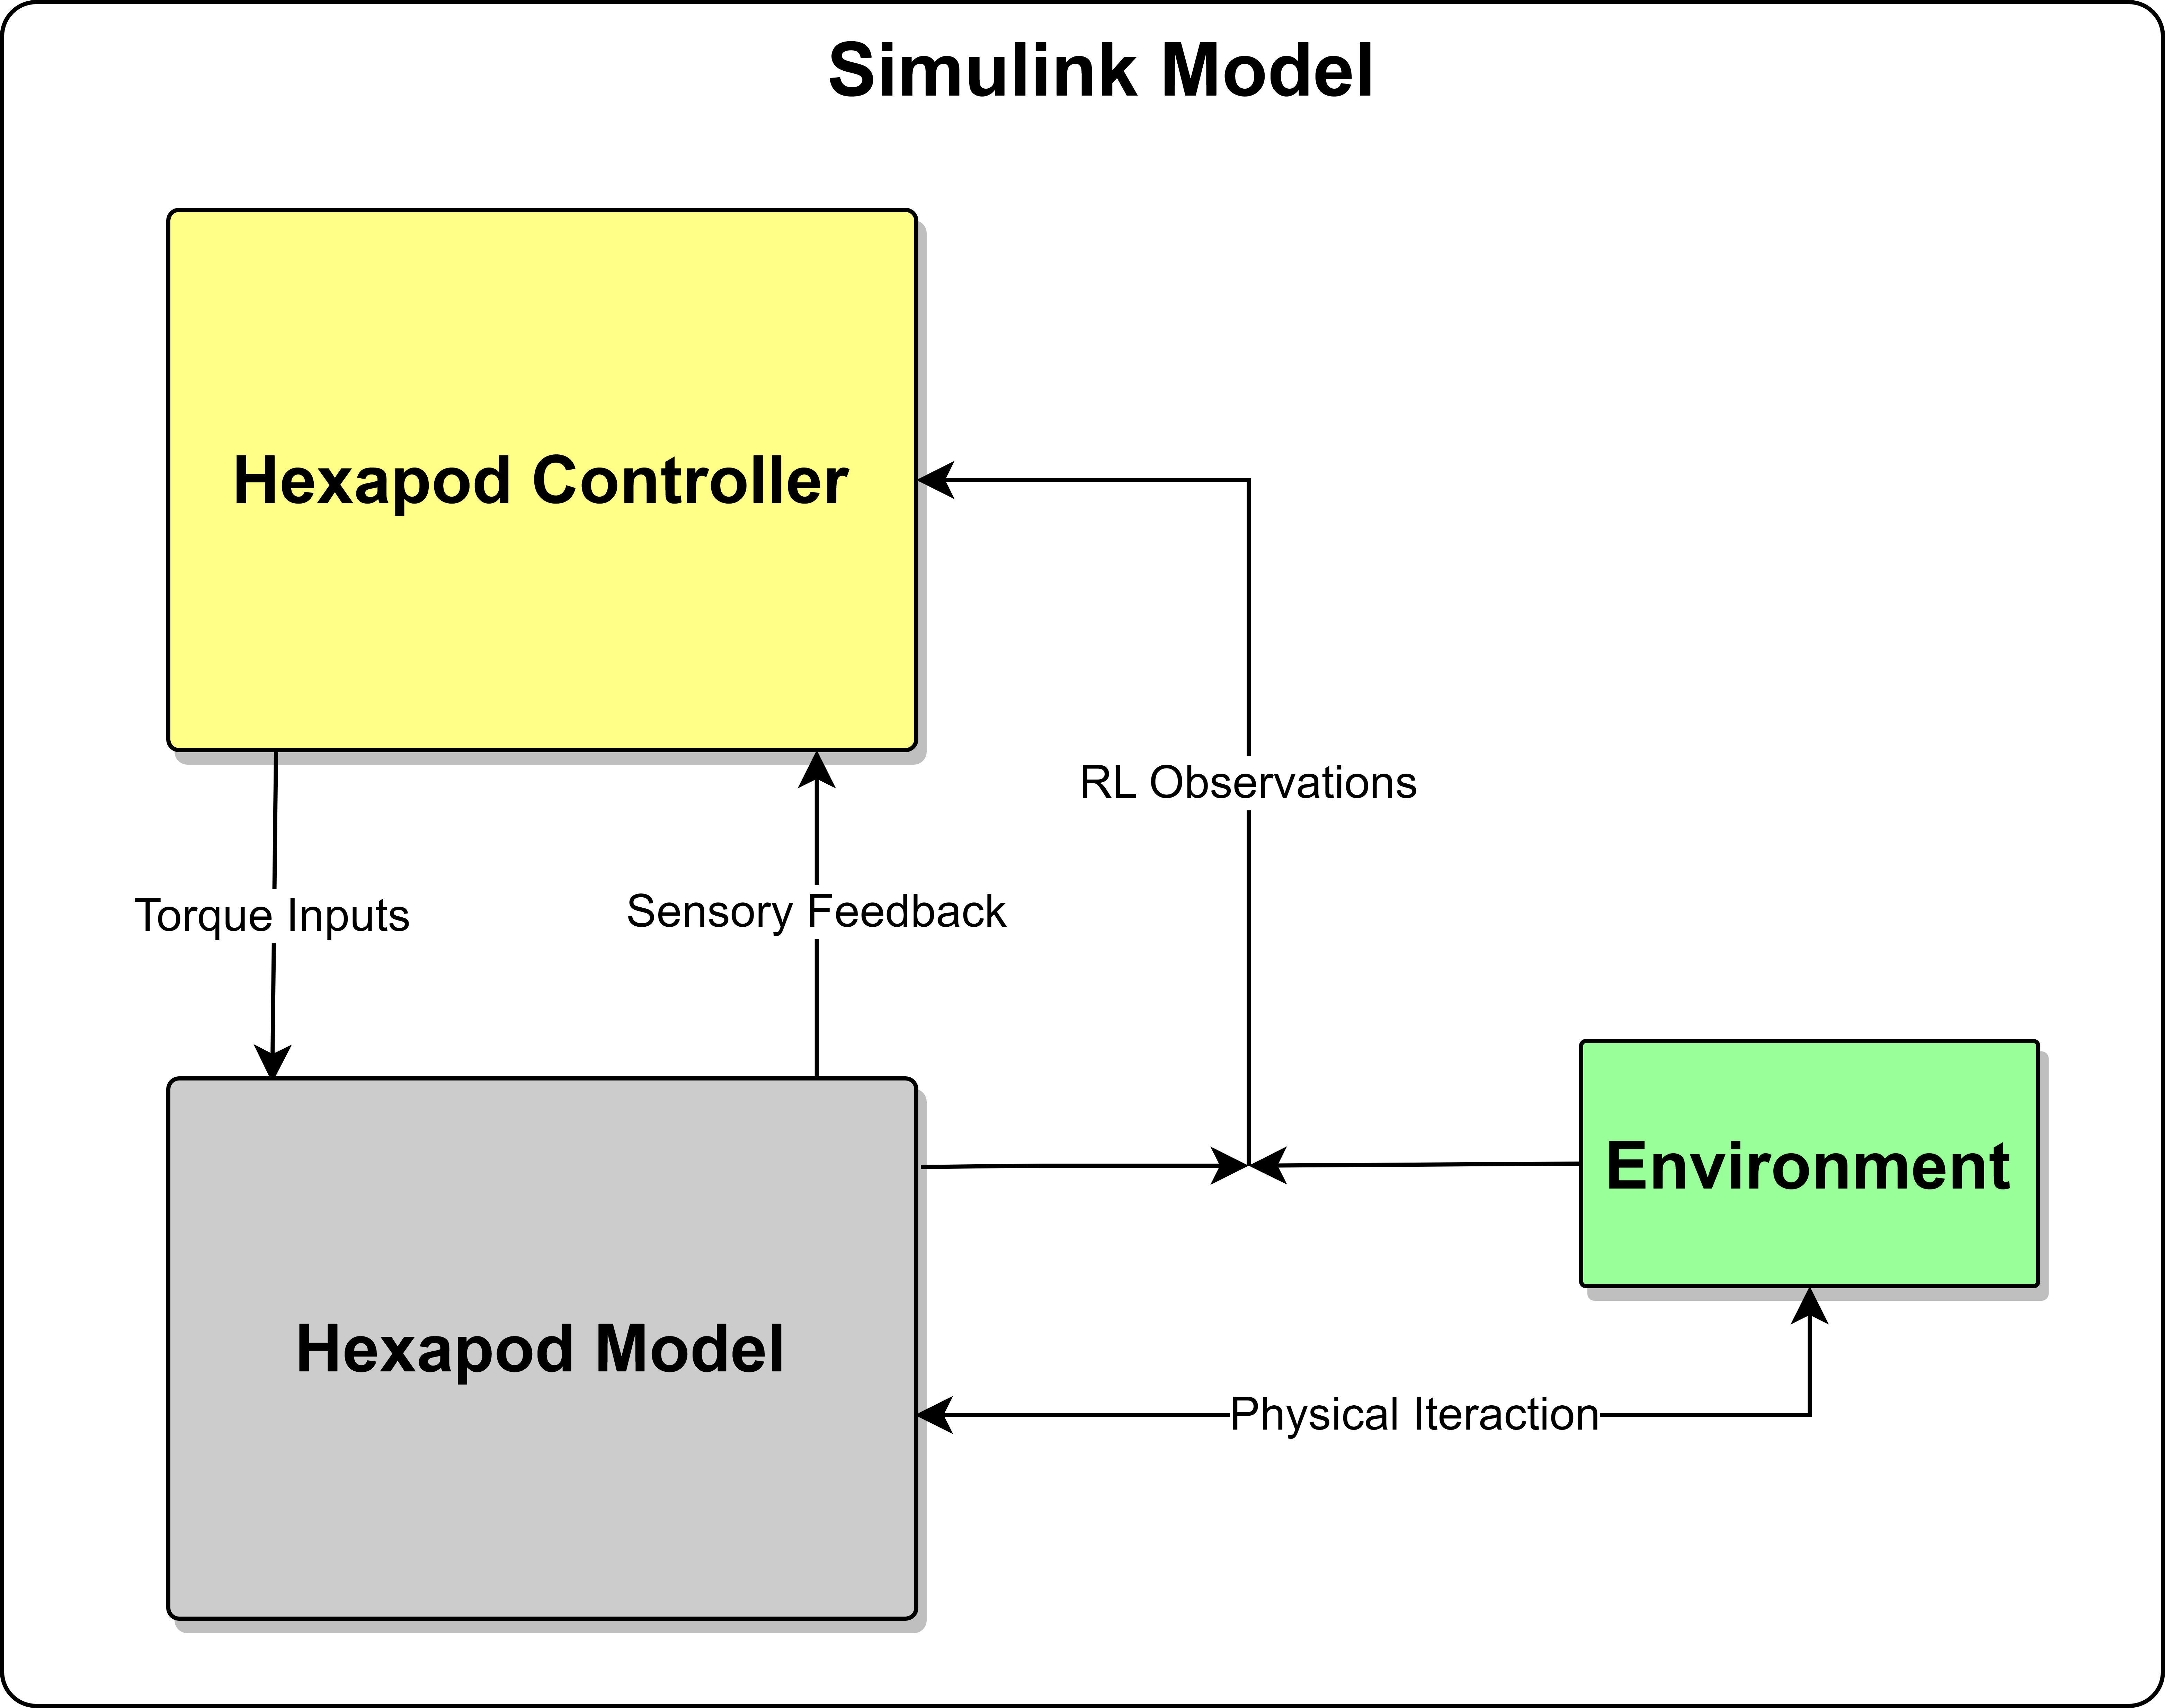
\includegraphics[scale=0.035]{HexapodModel_Overview}}
	\caption{Simulink Model Overview}
	\label{figure: Simulink Model Overview}
\end{figure}

\subsection{Model of the Hexapod}

\begin{figure}
	\centerline{\includesvg[scale=0.7]{Simulink/Simulink_PhysicalHexapodOverview}}
	\caption{Hexapod Model Overview}
	\label{figure: Hexapod Model Overview}
\end{figure}

\begin{figure}
	\centerline{\includesvg[scale=0.6]{Simulink/Simulink_HexapodLegOverview}}
	\caption{Model of Hexapod Leg}
	\label{figure: Hexapod Leg}
\end{figure}


The hexapod model we developed in this thesis is based on the \textit{PhantomX MK4} hexapod developed by \textit{Trossen Robotics}.
A digital model of this robot is provided by the company in the form of a .urdf file which can be obtained from their Github page \parencite{interbotixGithub}.
\textbf{U}nified \textbf{R}obotics \textbf{D}escription \textbf{F}ormat is a common format to describe the physical and kinematic properties of a robot or robotic component. 
It defines the way in which links and joints are connected, the general geometry of the robot as well as visual and collision geometry.
The geometry is provided in a separate folder of CAD-files which define the leg links and body structure as 
polygon meshes and are referenced in the urdf.
We use MATLABs capability to convert the urdf file into a Simscape-based Simulink model.
The resulting model consists of Simscape joints, rigid transforms and rigid bodies to represent the links.
The 3D-model off the hexapod can be seen in Fig. \ref{figure: PhantomX 3D model}.


\begin{figure}[]
	\begin{subfigure}{.5\textwidth} % this sets the figure to be max half the width of the page
		\centering
		% include first image
		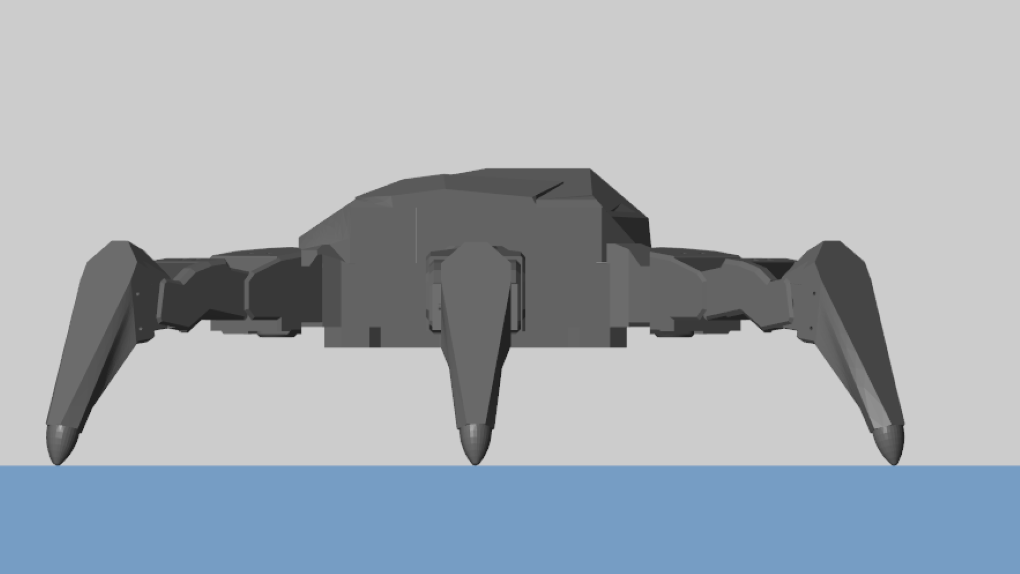
\includegraphics[width=.9\linewidth]{PhantomX_MK4_SideView}  % this sets the image to fill 90% of the available space -> 45% of the line width in total. 
		\caption{}
		\label{figure: PhantomX Side View}
	\end{subfigure}
	\begin{subfigure}{.5\textwidth}
		\centering
		% include second image
		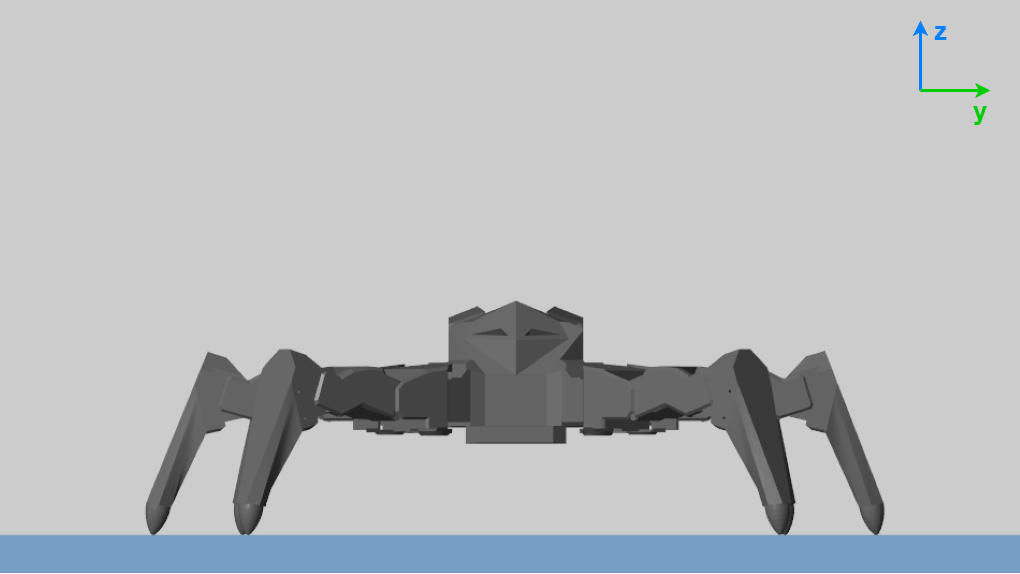
\includegraphics[width=.9\linewidth]{PhantomX_MK4_FrontView}  
		\caption{}
		\label{figure: PhantomX Front View}
	\end{subfigure}
	
	\label{fig:fig}
	\begin{subfigure}{\textwidth}
		\centering
		% include third image
		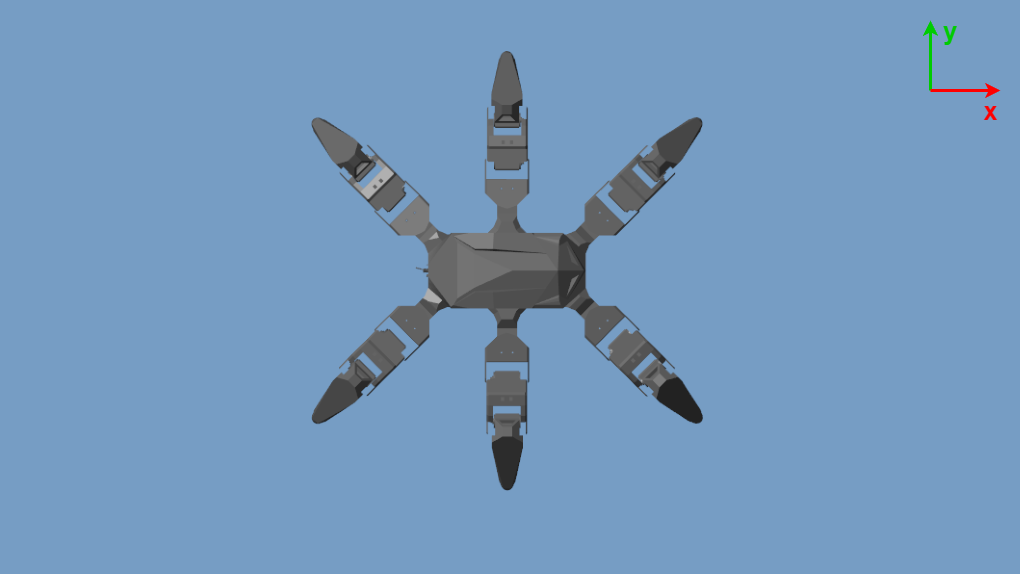
\includegraphics[width=.45\linewidth]{PhantomX_MK4_TopView}   % this width should be half of the width of the other two images
		\caption{}
		\label{figure: PhantomX Top View}
	\end{subfigure}
	\caption[]{3D model of Trossen Robotix PhantomX MK4}
	\label{figure: PhantomX 3D model}
\end{figure}
\todo{get each image into list of figures, but exclude complete figure}

From a top level perspective, the hexapod model consists of the main body(thorax) and its 6 legs.
This system receives as input the torque to be applied on each joint and outputs sensory data taken from these joints, namely the joints position, velocity and acceleration.
The main body of the hexapod robot is represented by a rigid body and a main coordinate frame.
Each of the robots legs consists of 3 rigid bodies(coxa, femur and tibia) which are connected to each other by 2 joints.
A third joint then attaches the coxa and the leg as a whole to the main body.
Each of the joints used has 1 (rotational) DoF.
To position each rigid body and joint correctly, rigid transformations are used to translate and rotate each component.

As mentioned above, joints can receive as input a torque to be applied and can output sensory data, such as the joints position, velocity and acceleration. 
To simplify the model, we did not model the physical servo motors and instead used this direct torque input to actuate the joints.

The internal joint parameters are given in table \ref{table: Joint parameters}.
Some of these parameters are adapted from \parencite{FIND AUTHOR} and some were automatically imported by MATLAB from the urdf specification.

\begin{table}
	\centering
	\begin{tabular}{| l | c |}
		\hline
		\textbf{parameter} & \textbf{value} \\
		\hline
		spring stiffness & 0 \\
		\hline
		damping coefficient & 0 \\
		\hline
		spring stiffness(joint boundary) & $10^4 \frac{Nm}{\text{deg}}$ \\
		\hline
		damping coefficient(joint boundary) &  $10 \frac{Nm \cdot s}{\text{deg}}$\\
		\hline
		transit region width(joint boundary) &  $10^{\circ}$\\
		\hline
	\end{tabular}
	\caption{Internal joint parameters}
	\label{table: Joint parameters}
\end{table}


In this thesis we only utilize the sensor information about the current joint positions, but to allow for further expansions on the model, such as optimizing for minimal energy consumption, joint velocity and acceleration are provided as well.
It should be noted, that integrating the joint position over time would implicitly yield the same result, but we decided for ease of use to include this data explicitly.

To encapsulate the system and only provide the necessary inputs and outputs, the hexapod model is placed inside a subsystem.
This also allows for the duplication of the hexapod system, so that in future research it is possible to use this system in multi-agent simulations as well.


\subsection{Environment}
To validate the robot model and to provide a place for the robot to learn the coordination rules of its legs, we constructed a simple test environment.
The environment currently only consists of a horizontal plane, but can expanded to include more complex terrain with little effort.
Some examples which we experimented with but did not include in this thesis are inclined planes and also small obstacles on the ground.
As Simscape itself only provides basic geometric objects but allows for the use .stl files to define the shape of objects, complex terrain such as irregular, uneven surfaces can be imported with relative ease.

In addition to being the testing ground of the hexapod model, the environment also acts as part of the reinforcement learning process.
Similar to \ref{figure: RL Illustration}, the environment provides observations to the RL agent and calculates a reward signal, based on the agents performance.
It does not directly receive actions from the agent, as the hexapod to which the actions are applied is its own subsystem.
If we would define the environment exactly like \ref{figure: RL Illustration,}, we would have to include both the environment subsystem and the hexapod subsystem as part of the "RL" environment.
For obvious reasons such as modularity and clarity of model we chose not to adapt this.

\subsection{Controller}
The controller is responsible for the hexapods locomotion.
It controls the movement of the robots six legs according to a predefined gait.
As inputs, the controller receives the sensory data from the hexapod model.
According to this data the controller outputs the torques to be applied to each joint.

\begin{figure}
	\centerline{\includegraphics[scale=0.03]{HexapodController}}
	\caption{Controller Overview}
	\label{figure: Controller Overview}
\end{figure}
Each of the hexapods legs is controlled by a separate control unit which receives the information of the legs joint sensors as input and computes the torques to be applied to its joints as output.
The control unit for a leg receives the frequency for the swing-stance cycle, duty-percentage of the swing phase and swing-initiation signal as coordination inputs.
This information can either come from a static gait definition, in which the parameters for each leg are statically configured, or can be provided by a reinforcement learning agent.
The agent receives observations from the environment and hexapod model as well as a reward signal and outputs actions in the form as mentioned above.

\begin{figure}
	\centerline{\includesvg[scale=0.6]{Simulink/Simulink_LegControllerOverview}}
	\caption{Control unit for a single leg}
	\label{figure: Leg control unit}
\end{figure}

A single leg control unit, as seen in \ref{figure: Leg control unit}, consists of a leg trajectory generator and one PID feedback control loop for each of the 3 leg joints.
The leg trajectory generator is responsible for generating a path for the leg to follow according to the input frequency, duty cycle swing initiation and pattern rotation.
It outputs the desired angle for the \textalpha-, \textbeta- and \textgamma-joints, which the PID controllers are then trying to achieve.
The PID controller parameters $K_p$, $K_i$ and $K_d$ (and $N$) are tuned via trial-and-error method and are depicted in \ref{table: PID parameters}.

\begin{figure}
	\centerline{\includesvg[scale=0.75]{Simulink/Simulink_LegTrajectoryGenerationOverview}}
	\caption{Leg trajectory generator}
	\label{figure: Leg trajectory generator}
\end{figure}

The leg trajectory generator, as seen in \ref{figure: Leg trajectory generator}, consists of a signal generator, a pattern rotation subsystem and an analytic inverse kinematics solver.
The signal generator is responsible for creating a continuous leg trajectory given as x- and z-coordinates.
The pattern rotation subsystems rotates, if required, the x-z-trajectory around the z-axis to allow for omni-directional movement of the robot.
At the end of the trajectory generation the inverse kinematics block receives the trajectory coordinates and translates them into joint angles.
Even though Simulinks \textit{Robotics System Toolbox} includes an iterative IK-solver, we decided to implement our own analytical solver to increase simulation speed.
Due to the nature of an iterative solver, the calculation time required is significantly higher than that of a purpose-build analytical solver, in our case about x to y times faster.

\begin{figure}
	\centerline{\includesvg[scale=0.85]{Simulink/Simulink_SignalGeneratorOverview}}
	\caption{Signal Generator}
	\label{figure: Signal Generator}
\end{figure}

A Signal Generator, as seen in \ref{figure: Signal Generator}, consists two parts, a swing phase subsystem and a stance phase subsystem.
The stance subsystems provide the x- and z-coordinate signal during stance, the swing subsystem during swing.
The coordination between these two units is influenced by the cycle frequency, duty factor and swing initiation signal.
If the swing initiation is pulled high, the swing phase subsystem is reset(so it starts from the beginning) and the outputs(x,z) are switched to the swing system.
When the swing phase is finished, meaning the x-coordinate coincides with the AEP, the swing phase subsystem gives up control the the stance phase subsystem via the \textit{Swing finished} signal.
This induces a reset on the stance phase subsystem and switches the outputs over to this system.

\begin{figure}
	\centering
	\begin{subfigure}[b]{0.55\textwidth}
		\includesvg[width=1\linewidth]{Simulink/Simulink_SwingPhaseGenOverview}
		\caption{}
		\label{fig:Ng1} 
	\end{subfigure}
	
	\begin{subfigure}[b]{0.55\textwidth}
		\includesvg[width=1\linewidth]{Simulink/Simulink_SwingPhaseGenOverview}
		\caption{}
		\label{fig:Ng2}
	\end{subfigure}
	
	\caption[Swing and Stance Phase]{(a) Swing phase subsystem. The swing ellipse is generated by two sine waves with different amplitude and phase. (b) Stance phase subsystem. As opposed to (a), the x-coordinate is now generated by a linear function and the z-coordinate is 0 throughout the whole phase.
		values of $M,I$.}
\end{figure}




\begin{table}
	\centering
	\begin{tabular}{| c | c |}
		\hline
		parameter & value\\
		\hline
		$K_p$ & ... \\
		\hline
		$K_i$ & ... \\
		\hline
		$K_d$ & ... \\
		\hline
		$N$ & ... \\
		\hline
	\end{tabular}
	\caption{Gain parameters used for pid-tuning}
	\label{table: PID parameters}
\end{table}

\begin{table}
	\centering
	\begin{tabular}{| c | c | c | c |} 
		\hline
		 & \textbf{\textalpha} & \textbf{\textbeta} & \textbf{\textgamma} \\ [0.5ex] 
		\hline
		left front, right back & 45 & 14.03624347 & 60.58440117  \\ 
		\hline
		left/right middle & 0 & 14.03624347 & 60.58440117 \\
		\hline
		right front, left back & -45 & 14.03624347 & 60.58440117 \\
		\hline
	\end{tabular}
	\caption{Initial joint positions according to urdf-file}
	\label{table:Initial joint positions}
\end{table}




\todo{Viel tiefer ins Detail gehen}
\todo{Bilder}

\section{Learning Leg Coordination}
The leg coordination problem can be considered a Markov decision process(MDP).
The MDP is a 5-tuple $\mathcal{\{S,A,P,R,\gamma\}}$, where $\mathcal{S}$ is a finite set of states, $\mathcal{A}$ is a finite set of actions, $\mathcal{P}$ is a state-transition probability matrix ($\mathcal{P}_{ss'}^a=\mathbb{P}[S_{t+1}=s' | S_t=s, A_t=a]$), $\mathcal{R}_s^a$ is a reward function ($\mathcal{R}_s^a = \mathbb{E}[R_{t+1} | S_t=s, A_t=a]$) and $\gamma \in [0,1]$ is a discount factor.



When we first started working on te RL process, te result were not very promising. The agent did stabilize, meaning it did not jump around randomly, but it was not able to find an efficient gain.
The agent never learned to reliably move a leg forward if it was start to drag behind due to reaching the PEP.

The reward stayed relatively flat over a period of over 2000 episodes of training.
The strong deviation from the mean, even after several hundred episodes can be attributed to an averaging window of just 5 episodes(or steps ?). 
In later training experiments, this averaging window was increased.
The small averaging window might have contributed to the poor performance of the agent.

DDPG does not jitter at start of learning, PPO does.


Start learning process of PPO(Proximal Policy Optimization) agent at a small step size(0.00025s = 0.25ms) to prevent simulation errors due to initial random jerking of robot legs.
After the agent has stabilized, the step size can be increased to speed up the further learning process.]



